\documentclass[preview]{standalone}
\usepackage{amssymb} 
\usepackage{amsthm}
\usepackage{mathtools}
\usepackage{bm}
\usepackage{xcolor}
\usepackage{standalone}


\newtheorem{theorem}{Theorem}


\renewcommand\qedsymbol{$\blacksquare$}


\begin{document}


% ============================== 1.01 Theorem 1601 ================================
\section{The sum of two odd integers is even.}
\begin{figure}[h!]
    \centering
    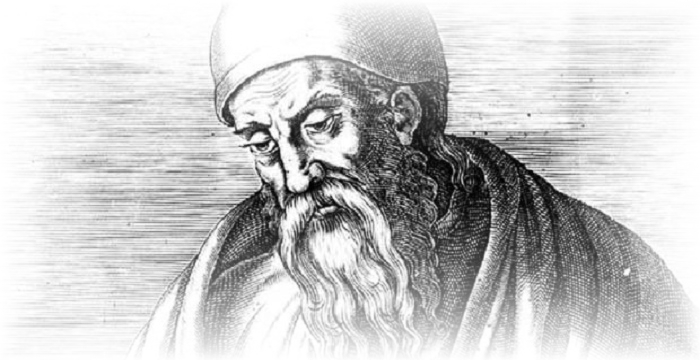
\includegraphics[width=12cm]{../resources/jpg/1.6.introduction.to.proofs/euclid.jpg}
    \caption*{\emph{Euclid.}}
\end{figure} 
\documentclass[preview]{standalone}
\usepackage{amssymb, amsthm}
\usepackage{mathtools}
\usepackage{bm}
\usepackage{xcolor}


\newtheorem{theorem}{Theorem}
\renewcommand\qedsymbol{$\blacksquare$}


\begin{document}
    
\begin{theorem} %[\textbf{1601}]
    Let \bm{$\chi$} and \bm{$\zeta$} be integers. 
    If \bm{$\chi$} and \bm{$\zeta$} are odd, 
    then \bm{$\chi + \zeta$} is even.
\end{theorem}

\begin{proof}
    By the definition for odd numbers, 
    there exists integers \bm{$\mu$} and \bm{$\nu$} such that 
    \bm{$\chi = 2\mu + 1$} and \bm{$\zeta = 2\nu + 1$}. 
    Hence,
    \begin{equation*}
        \chi + \zeta 
            = 
        \Big[
            \big \langle 2 \mu + 1 \big \rangle 
                + 
            \big \langle 2 \nu + 1 \big \rangle
        \Big]
            = 
        \Big[
            2 \big \langle \mu + \nu + 1 \big \rangle
        \Big]
    \end{equation*} 
    Integers are closed under addition. 
    Thus, the factor 
    \bm{$\big \langle \mu + \nu + 1 \big \rangle$} is an integer. 
    It follows that \bm{$\chi + \zeta$} is even, 
    by the definition for even numbers.
\color{lightgray} \end{proof}

\end{document}
\pagebreak


% ============================== 1.02 Theorem 1602 =================================
\section{The sum of two even integers is even.}
\documentclass[preview]{standalone}
\usepackage{amssymb, amsthm}
\usepackage{mathtools}
\usepackage{bm}


\newtheorem{theorem}{Theorem}
\renewcommand\qedsymbol{$\blacksquare$}


\begin{document}

\begin{theorem} %[\textbf{1602}]
    Let \bm{$\chi$} and \bm{$\zeta$} be integers. 
    If \bm{$\chi$} and \bm{$\zeta$} are even, 
    then \bm{$\chi \textbf{ + } \zeta$} is even.
\end{theorem}

\begin{proof}
    By the definition for even numbers, 
    there exist integers \bm{$\mu$} and \bm{$\nu$} such that 
    \bm{$2\mu \textbf{ = } \chi$} and \bm{$2\nu \textbf{ = } \zeta$}. 
    Hence,
    \begin{equation*}
        \chi + \zeta 
            = 
        \Big[
            \big \langle 2\mu \big \rangle
                + 
            \big \langle 2\nu \big \rangle
        \Big]
            =
        \Big[ 
            2 \big \langle \mu + \nu \big \rangle
        \Big]
    \end{equation*} 
    Integers are closed under addition. 
    Thus, the factor 
    \bm{$\big \langle \mu \textbf{ + } \nu \big \rangle$} 
    is an integer. 
    It follows that \bm{$\chi \textbf{ + } \zeta$} is even, 
    by the definition for even numbers.
\end{proof}

\end{document}
\sep


% ============================== 1.03 Theorem 1603 =================================
\section{The square of an even number is even.}
\documentclass[preview]{standalone}
\usepackage{amssymb, amsthm}
\usepackage{mathtools}
\usepackage{bm}
\usepackage{xcolor}


\newtheorem{theorem}{Theorem}
\renewcommand\qedsymbol{$\blacksquare$}


\begin{document}
    
\begin{theorem} %[\textbf{1603}]
    If \bm{$\chi$} is an even integer, 
    then \bm{$\chi^2$} is an even integer.
\end{theorem}

\begin{proof}
    By the definition for even numbers, 
    there exists an integer \bm{$\eta$} such that 
    \bm{$\chi = 2\eta$}. 
    Hence,
    \begin{equation*}
        \big \langle 2 \eta \big \rangle ^2 
            = 
        4 \eta ^2 
            = 
        2 \big \langle 2 \eta ^2 \big \rangle
    \end{equation*}
    Integers are closed under multiplication. 
    Thus, the factor 
    \bm{$\big \langle 2 \eta ^2 \big \rangle$} is an integer. 
    It follows that \bm{$\chi^2$} is even, by 
    the definition for even numbers.
\color{lightgray} \end{proof}

\end{document}
\sep


% ============================== 1.04 Theorem 1604 =================================
\section{The additive inverse of an even number.}
\documentclass[preview]{standalone}
\usepackage{amssymb, amsmath, amsthm}
\usepackage{mathtools}
\usepackage{bm}


\newtheorem{theorem}{Theorem}
\renewcommand\qedsymbol{$\blacksquare$}


\begin{document}


\begin{theorem} %[\textbf{1604}]
    The additive inverse of an even number is an even number.
\end{theorem}

\begin{proof}
    Let \bm{$\chi$} be an even number. 
    There exists an integer \bm{$\eta$} such that 
    \bm{$\chi \textbf{ = } 2\eta$}, 
    by the definition for even numbers. 
    The additive inverse for \bm{$\chi$} is,
    \begin{equation*}
        -1 \big \langle \chi \big \rangle
            = 
        -1 \big \langle 2 \eta \big \rangle
    \end{equation*} 
    By commutativity of multiplication that is,
    \begin{equation*}
        -1 \big \langle 2 \eta \big \rangle
            = 
        2 \big \langle - \eta \big \rangle
    \end{equation*}
    Since integers are closed under multiplication, 
    the factor \bm{$\big \langle \textbf{ - } \eta \big \rangle$} is an integer. 
    It follows that the additive inverse of \bm{$\chi$} is an even number, 
    by the definition for even numbers.
\end{proof}


\end{document} 
\pagebreak


% ============================== 1.05 Theorem 1605 =================================
\section{Special even parity.}
\documentclass[preview]{standalone}
\usepackage{amssymb, amsthm}
\usepackage{mathtools}
\usepackage{bm}
\usepackage{xcolor}


\newtheorem{theorem}{Theorem}
\renewcommand\qedsymbol{$\blacksquare$}


\begin{document}


\begin{theorem} %[\textbf{1605}]
    Let \bm{$\mu$}, \bm{$\zeta$}, and \bm{$\pi$} be integers. 
    If \bm{$\mu + \zeta$} and \bm{$\zeta + \pi$} are even, 
    then \bm{$\mu + \pi$} is even.
\end{theorem}

\begin{proof}
    By the hypothesis, 
    there exist integers \bm{$\sigma$} and \bm{$\epsilon$} such that 
    \bm{$\mu + \zeta = 2\sigma$}, 
    and \bm{$\zeta + \pi = 2\epsilon$}. 
    Hence, 
    \begin{equation*}
        \big \langle \mu + \zeta \big \rangle 
            + 
        \big \langle \zeta + \pi \big \rangle
            = 
        2 \sigma + 2 \epsilon
    \end{equation*}
    Subtracting \bm{$2\zeta$} from both sides, 
    by the subtraction property of equality for equations, 
    produces
    \begin{equation*}
        \Big \langle \mu + \pi \Big \rangle
            = 
        \Big \langle 2 \sigma + 2 \epsilon - 2 \zeta \Big \rangle
            = 
        \Big[ 2 \big \langle \sigma + \epsilon - \zeta \big \rangle \Big]
    \end{equation*}
    \bm{$\sigma$} and \bm{$\epsilon$} are integers,
    by the definition for even numbers, 
    and \bm{$\zeta$} is an integer by the hypothesis. 
    Since addition and subtraction are closed on integers, 
    the factor 
    \bm{$\big \langle \sigma + \epsilon - \zeta \big \rangle$} 
    is an integer. 
    It follows that \bm{$\mu + \pi$} is an even, 
    by the definition for 
    even numbers.
\color{lightgray} \end{proof}


\end{document}
\begin{center}
    
\includegraphics[width=6cm]{../resources/jpg/1.6.introduction.to.proofs/olympics.jpg}
\end{center}


% ============================== 1.06 Theorem 1606 =================================
\section{The product of two odd numbers is odd.}
\documentclass[preview]{standalone}
\usepackage{amssymb, amsthm}
\usepackage{mathtools}
\usepackage{bm}
\usepackage{xcolor}


\newtheorem{theorem}{Theorem}
\renewcommand\qedsymbol{$\blacksquare$}


\begin{document}


\begin{theorem} %[\textbf{1606}]
    The product of two odd numbers is odd.
\end{theorem}

\begin{proof}
    Suppose that \bm{$\mu$} and \bm{$\zeta$} are odd numbers. 
    By the definition for odd numbers, 
    there exist integers \bm{$\sigma$} and \bm{$\epsilon$} such that 
    \bm{$\mu = 2\sigma + 1$} and \bm{$\zeta = 2\epsilon + 1$}. 
    Thus, the product of odd numbers \bm{$\mu \zeta$} is,
    \begin{equation*}
        \mu \zeta 
            =
        \Big[ 
            \big \langle 2 \sigma + 1 \big \rangle 
            \big \langle 2 \epsilon + 1 \big \rangle
        \Big]
            = 
        \Big[% \langle
            2 \sigma 2 \epsilon + 2 \sigma + 2 \epsilon + 1 
        \Big]% \rangle
            = 
        \Big[
            2 \big \langle 
                \sigma \epsilon + \sigma + \epsilon 
            \big \rangle 
                + 1
        \Big]
    \end{equation*}     
    The factor 
    \bm{$\big \langle \sigma \epsilon + \sigma + \epsilon \big \rangle$} 
    is an integer because \bm{$\sigma$} and \bm{$\epsilon$} are integers by definition, 
    and integers are closed on addition. 
    Therefore, \bm{$\mu \zeta$} is odd by the definition for odd numbers.
\color{lightgray} \end{proof}


\end{document}
\pagebreak


% ============================== 1.07 Theorem 1608 =================================
\section{Two plus a perfect square is not perfect.}
\documentclass[preview]{standalone}
\usepackage{amssymb, amsthm}
\usepackage{mathtools}
\usepackage{bm}


\newtheorem{theorem}{Theorem}
\renewcommand\qedsymbol{$\blacksquare$}


\begin{document}


\begin{theorem} %[\textbf{1608}]
    If \bm{$\eta$} is a perfect square, 
    then \bm{$\eta \textbf{ + } 2$} is not a perfect square.
\end{theorem}

\begin{proof}
    Let \bm{$\eta$} be a perfect square. 
    Assume \bm{$\eta \textbf{ + } 2$} is a perfect square for the purpose of contradiction. 
    By the definition of perfect square, 
    \bm{$\sqrt{\eta}$} has to be an integer, 
    and by our assumption there exists an integer \bm{$\zeta$} such that 
    \bm{$\zeta^2 \textbf{ = } \eta \textbf{ + } 2$}. 
    So the equivalence 
    \bm{$\zeta^2 \textbf{ - } \big \langle \sqrt{\eta} \big \rangle ^2 \textbf{ = } 2$} 
    must be the difference of squares 
    \begin{equation*}
        \big \langle \zeta + \sqrt{\eta} \big \rangle 
        \big \langle \zeta - \sqrt{\eta} \big \rangle 
            =
        2
    \end{equation*}
    Since integers are closed on addition and subtraction, 
    it follows that the factors of \bm{$2$}, 
    \bm{$\big \langle \zeta \textbf{ + } \sqrt{\eta} \big \rangle$} and 
    \bm{$\big \langle \zeta \textbf{ - } \sqrt{\eta} \big \rangle$}, 
    have to be integers. 
    Because \bm{$2$} is prime, those integer factors can only be elements in the set
    \bm{$\{-2, -1, 1, 2\}$}. Thus, there are exactly two possibilities:
    \\ \\ \indent \indent \bm{$(i)$} $\zeta ^2 \textbf{ - } \big \langle \sqrt{\eta} \big \rangle ^2 \textbf{ = } 
                            \big \langle 2 \big \rangle \big \langle 1 \big \rangle$,
    \\ \indent \indent or \bm{$(ii)$} $\zeta ^2 \textbf{ - } \big \langle \sqrt{\eta} \big \rangle ^2 \textbf{ = } 
                            \big \langle -1 \big \rangle \big \langle -2 \big \rangle.$
    \\ \\ In case \bm{$(i)$}, without loss of generality, 
    we have a system of linear equations in two variables \bm{$\zeta$} and \bm{$\sqrt{\eta}$}:
    \begin{equation*}
        \zeta + \sqrt{\eta} = 2
    \end{equation*}
    \begin{equation*}
        \zeta - \sqrt{\eta} = 1
    \end{equation*}
    The matrix of coefficients 
    $\bm{\Psi \textbf{ = }} \left[\begin{smallmatrix}
        \bm{1} & \bm{1} \\
        \bm{1} & \bm{-1} 
    \end{smallmatrix}\right]$, 
    the inverse for which is
    $\bm{\Psi^{-1} \textbf{ = }} \left[\begin{smallmatrix}
        \bm{0.5} & \bm{0.5} \\
        \bm{0.5} & \bm{-0.5}
    \end{smallmatrix}\right]$. 
    The product of \bm{$\Psi^{-1}$} and the matrix of solutions yields \bm{$\zeta \textbf{ = } 1.5$}, 
    which is not in \bm{$\mathbb{Z}$}; 
    contradicting the assumption that \bm{$\zeta^2$} was a perfect square.
    \\ \\ 
    In case \bm{$(ii)$}, 
    we are presented with a similar system of linear equations. 
    The only difference in this system compared to \bm{$(i)$} is the matrix of solutions 
    $\bm{\Phi \textbf{ = }} \left[\begin{smallmatrix}
        \bm{-1} \\
        \bm{-2}
    \end{smallmatrix}\right]$. 
    \bm{$\Psi^{-1}\Phi$} yields \bm{$\zeta \textbf{ = } -1.5$}, 
    which is not in \bm{$\mathbb{Z}$}, 
    a contradiction. 
    Thus, the assumption that \bm{$\zeta^2$} was a perfect square must be false in this case, as well.
    \\ \\
    Since the assumption proves false in all possible cases, 
    it is not possbile that both \bm{$\eta \textbf{ + } 2$}, and \bm{$\eta$} are perfect squares.
\end{proof}


\end{document}
\vspace{1.5\baselineskip}
\sep
\pagebreak


% ============================== 1.08 Theorem 1609 =================================
\section{The sum of irrational and rational is irrational.}
\documentclass[preview]{standalone}
\usepackage{amssymb, amsthm}
\usepackage{mathtools}
\usepackage{bm}
\usepackage{xcolor}


\newtheorem{theorem}{Theorem}
\renewcommand\qedsymbol{$\blacksquare$}


\begin{document}


\begin{theorem} %[\textbf{1609}]
    The sum of an irrational number and a rational number is irrational.
\end{theorem}

\begin{proof}
    By contradiction. Suppose that \bm{$\mu$} and \bm{$\zeta$} are rational numbers, 
    and let \bm{$\chi$} be an irrational number. 
    For the purpose of contradiction, 
    assume the negation of the hypothesis. 
    That is, the proposition 
        $$\lnot p: \emph{the sum of an irrational number and a rational number 
        is rational.}$$
    Hence, \bm{$\chi + \mu = \zeta$}, 
    by the assumption \bm{$\lnot p$}. 
    Thus, 
    \bm{$\chi = \zeta + \big \langle - \mu \big \rangle$}, 
    by the additive equality property for equations. 
    But rational numbers are closed under addition by the closure property for rational numbers. 
    So \bm{$\lnot p$} implies \bm{$\chi$} is rational, 
    and \bm{$\chi$} is irrational; a contradiction.
\color{lightgray} \end{proof}


\end{document}
\begin{figure}[h!]
    \centering
    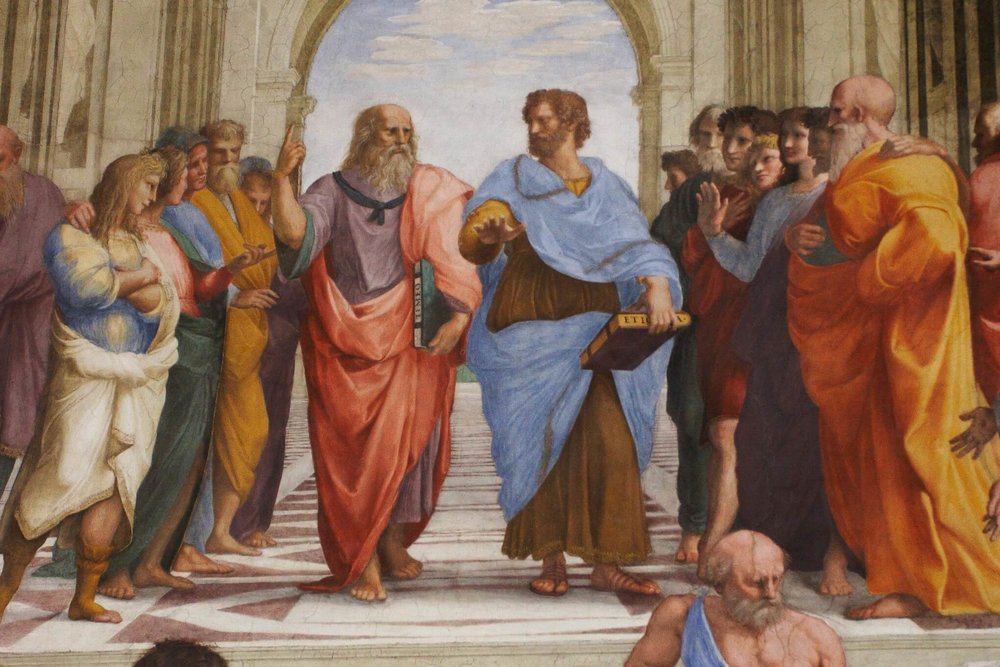
\includegraphics[width=12.5cm]{../resources/jpg/1.6.introduction.to.proofs/plato-republic.jpg}
    \caption*{\emph{Plato and Aristotle.}}
\end{figure}


% ============================== 1.09 Theorem 1610 ================================
\section{The product of two rational numbers is rational.}
\documentclass[preview]{standalone}
\usepackage{amssymb, amsthm}
\usepackage{mathtools}
\usepackage{bm}
\usepackage{xcolor}


\newtheorem{theorem}{Theorem}
\renewcommand\qedsymbol{$\blacksquare$}


\begin{document}


\begin{theorem} %[\textbf{1610}]
    The product of two rational numbers is rational.
\end{theorem}

\begin{proof}
    Let \bm{$\mu$} and \bm{$\zeta$} be rational numbers. 
    By the definition for rational numbers, 
    there exist integers \bm{$\alpha$}, \bm{$\beta$}, \bm{$\gamma$}, and \bm{$\delta$} such that 
    \bm{$\mu = \frac{\alpha}{\beta}$} and \bm{$\zeta = \frac{\gamma}{\delta}$}. 
    The product of \bm{$\mu$} and \bm{$\zeta$} is \bm{$\frac{\alpha\gamma}{\beta\delta}$}. 
    Since integers are closed under multiplcation, 
    \bm{$\alpha\gamma$} and \bm{$\beta\delta$} are integers. 
    Thus \bm{$\mu\zeta$} is rational by definition.
\color{lightgray} \end{proof}



\end{document}
\pagebreak


% ============================== 1.10 Theorem 1612 ================================
\section{The product of irrational and rational is irrational.}
\documentclass[preview]{standalone}
\usepackage{amssymb, amsthm}
\usepackage{mathtools}
\usepackage{bm}
\usepackage{xcolor}


\newtheorem{theorem}{Theorem}
\renewcommand\qedsymbol{$\blacksquare$}


\begin{document}


\begin{theorem} %[\textbf{1612}]
    The product of a nonzero rational number and an irrational number is 
    irrational.
\end{theorem}

\begin{proof}
    For the purpose of contradiction, assume the negation of the hypothesis; 
    the proposition 
        $$\lnot p : \emph{the product of a nonzero rational number and an 
        irrational number}$$
        $\indent \indent \indent \emph{is rational}$
        \\ \\
    Let \bm{$\alpha$}, \bm{$\beta$}, \bm{$\gamma$}, and \bm{$\delta$} be integers such that 
    \bm{$\alpha \neq 0$}, and let \bm{$\chi$} be an irrational number. 
    Then the proposition \bm{$\lnot p$} states 
    \begin{equation*}
        \Bigg(
            \frac{\alpha}{\beta} \space \cdot \space \chi 
        \Bigg)
            = 
        \Bigg(
            \frac{\gamma}{\delta}
        \Bigg)
    \end{equation*}    
    By the multiplicative equality property for equations, that is
    \begin{equation*}
        \Bigg(
            \chi
        \Bigg) 
            = 
        \Bigg(
            \frac{\gamma}{\delta} \space \cdot \space \frac{\beta}{\alpha} 
        \Bigg)
            =
        \Bigg( 
            \frac{\gamma\beta}{\delta\alpha}
        \Bigg)
    \end{equation*}
    By Theorem 9 (the closure property for multplication on rational numbers,) 
    \bm{$\chi$} is rational. 
    Thus, \bm{$\lnot p$} implies \bm{$\chi$} is rational and irrational.
\color{lightgray} \end{proof}
\

\end{document}
\sep


% ============================== 1.11 Theorem 1613 ================================
\section{The multiplicative inverse of an irrational number.}
\documentclass[preview]{standalone}
\usepackage{amssymb, amsthm}
\usepackage{mathtools}
\usepackage{bm}


\newtheorem{theorem}{Theorem}
\renewcommand\qedsymbol{$\blacksquare$}


\begin{document}


\begin{theorem} %[\textbf{1613}]
    If \bm{$\chi$} is an irrational number, 
    then \bm{$\frac{1}{\chi}$} is irrational.
\end{theorem}

\begin{proof}
    By the contrapositive. 
    Suppose that \bm{$\frac{1}{\chi}$} is a rational number. 
    By the definition for rational numbers, 
    there exist integers \bm{$\alpha$} and \bm{$\gamma$} such that 
    \bm{$\frac{1}{\chi} \textbf{ = } \frac{\alpha}{\gamma}$}. 
    Note that \bm{$\alpha$} is nonzero (because \bm{$\frac{1}{\chi}$} is nonzero.) 
    By the multiplicative property of equality for equations,
    \begin{equation*}
        \left\{
            \left(
                \chi \cdot \frac{1}{\chi}
            \right) 
                = 
            \left(
                \chi \cdot \frac{\alpha}{\gamma}
            \right)
        \right\} 
            \equiv
        \left\{
            \left(
                \frac{\chi}{\chi} \cdot \frac{\gamma}{\alpha}
            \right) 
                = 
            \left(
                \frac{\chi \alpha}{\gamma} \cdot \frac{\gamma}{\alpha}
            \right)
        \right\} 
            \equiv
        \bigg\{
            \frac{\gamma}{\alpha} 
                = 
            \chi
        \bigg\}
    \end{equation*}
    \bm{$\frac{\gamma}{\alpha} \textbf{ = } \chi$} is rational, 
    by definition. 
    Thus, if \bm{$\frac{1}{\chi}$} is rational, 
    then \bm{$\chi$} is rational.
\end{proof}


\end{document}
\pagebreak


% ============================== 1.12 Theorem 1614 ================================
\section{The multiplicative inverse of a rational number.}
\documentclass[preview]{standalone}
\usepackage{amssymb, amsthm}
\usepackage{mathtools}
\usepackage{bm}
\usepackage{xcolor}


\newtheorem{theorem}{Theorem}
\renewcommand\qedsymbol{$\blacksquare$}


\begin{document}


\begin{theorem} %[\textbf{1614}]
    If \bm{$\chi$} is a rational number and \bm{$\chi \neq 0$}, 
    then \bm{$\frac{1}{\chi}$} is rational.
\end{theorem}

\begin{proof}
    Let \bm{$\alpha$} and \bm{$\gamma$} be nonzero integers. 
    \bm{$\chi = \frac{\alpha}{\gamma}$}, 
    by the definition for rational numbers. 
    By the multiplicative property of equality for equations
    \begin{equation*}
        \left\{
            \left(
                \frac{1}{\chi} \cdot \chi
            \right) 
                = 
            \left(
                \frac{1}{\chi} \cdot \frac{\alpha}{\gamma}
            \right)
        \right\} 
            \equiv 
        \left\{
            \left(
                \frac{\chi}{\chi} \cdot \frac{\gamma}{\alpha}
            \right) 
                = 
            \left(
                \frac{\alpha}{\chi\gamma} \cdot \frac{\gamma}{\alpha}
            \right)
        \right\}
            \equiv 
        \left\{
            \frac{\gamma}{\alpha} 
                = 
            \frac{1}{\chi}
        \right\}
    \end{equation*}
    \bm{$\frac{\gamma}{\alpha} = \frac{1}{\chi}$} is rational, by definition. 
    Thus, if \bm{$\chi$} is a rational number and \bm{$\chi \neq 0$}, 
    then \bm{$\frac{1}{\chi}$} is rational.
\color{lightgray} \end{proof}
\

\end{document}
\begin{figure}[h!]
    \centering
    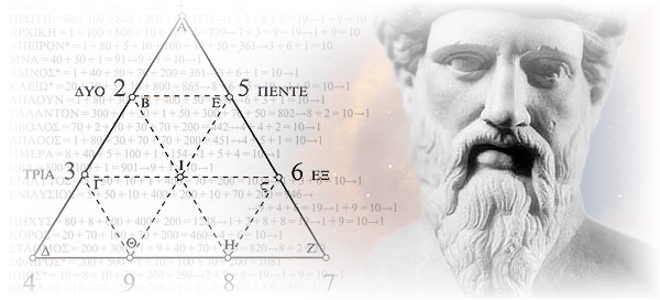
\includegraphics[width=13cm]{../resources/jpg/1.6.introduction.to.proofs/pythagoras.jpg}
    \caption*{\emph{Pythagoras.}}
\end{figure}


% ============================== 1.13 Theorem 1615 ================================
\section{A special corollary from additive compatibility.}
\documentclass[preview]{standalone}
\usepackage{amssymb, amsthm}
\usepackage{mathtools}
\usepackage{bm}


\newtheorem{theorem}{Theorem}
\renewcommand\qedsymbol{$\blacksquare$}


\begin{document}


\begin{theorem} %[\textbf{1615}]
    Let \bm{$\chi$} and \bm{$\zeta$} be real numbers. 
    If \bm{$\chi \textbf{ + } \zeta \ge 2$}, 
    then 
    \bm{$
        \big \langle \chi \ge 1 \big \rangle 
            \lor
    $}
    \\
    \bm{$
        \big \langle \zeta \ge 1 \big \rangle
    $}.
\end{theorem}

\begin{proof}
    By the contrapositive.
    Suppose the negation of the consequent: 
    \begin{equation*}
        \big \langle \chi < 1 \big \rangle 
            \land 
        \big \langle \zeta < 1 \big \rangle    
    \end{equation*}    
    By additive compatibility,
    \begin{equation*}
        \Big \langle \chi + \zeta \Big \rangle 
            < 
        \Big \langle 1 + 1 \Big \rangle 
            = 
        \Big \langle 
            2
        \Big \rangle
    \end{equation*}
    This is the logical negation of the direct hypothesis. Thus concludes the proof.
\end{proof}


\end{document}
\pagebreak


% ============================== 1.14 Theorem 1616 ================================
\section{Divisors of an even number.}
\documentclass[preview]{standalone}
\usepackage{amssymb, amsthm}
\usepackage{mathtools}
\usepackage{bm}
\usepackage{xcolor}


\newtheorem{theorem}{Theorem}
\renewcommand\qedsymbol{$\blacksquare$}


\begin{document}


\begin{theorem} %[\textbf{1616}]
    Let \bm{$\mu$} and \bm{$\zeta$} be integers. 
    If the product \bm{$\mu\zeta$} is even, 
    then \bm{$\mu$} is even or \bm{$\zeta$} is even.
\end{theorem}

\begin{proof}
    For the purpose of contraposition, suppose the negation of the consequent 
    \bm{$q$}
        $$\lnot q : \mu \text{ is odd and } \zeta \text{ is odd.}$$ 
    By definition, 
    there exist integers \bm{$\sigma$} and \bm{$\epsilon$} such that 
    \bm{$\mu = 2\sigma + 1$} and \bm{$\zeta = 2\epsilon + 1$}. 
    Thus, 
    \begin{equation*}
        \mu\zeta 
            =
        \Big[ 
            \big \langle 2 \sigma + 1 \big \rangle
            \big \langle 2 \epsilon + 1 \big \rangle 
        \Big]
            =
        \Big[ 
            2 
            \big \langle \sigma\epsilon + \sigma + \epsilon \big \rangle 
                + 
            1
        \Big]
    \end{equation*}
    The factor 
    \bm{$\big \langle \sigma \epsilon + \sigma + \epsilon \big \rangle$} 
    is an integer, 
    because integers are closed under addition and multiplication. 
    Thus, the product \bm{$\mu \zeta$} is odd, by definition.
\color{lightgray} \end{proof}
\

\end{document}
%\sep
\begin{figure}[h!]
    \centering
    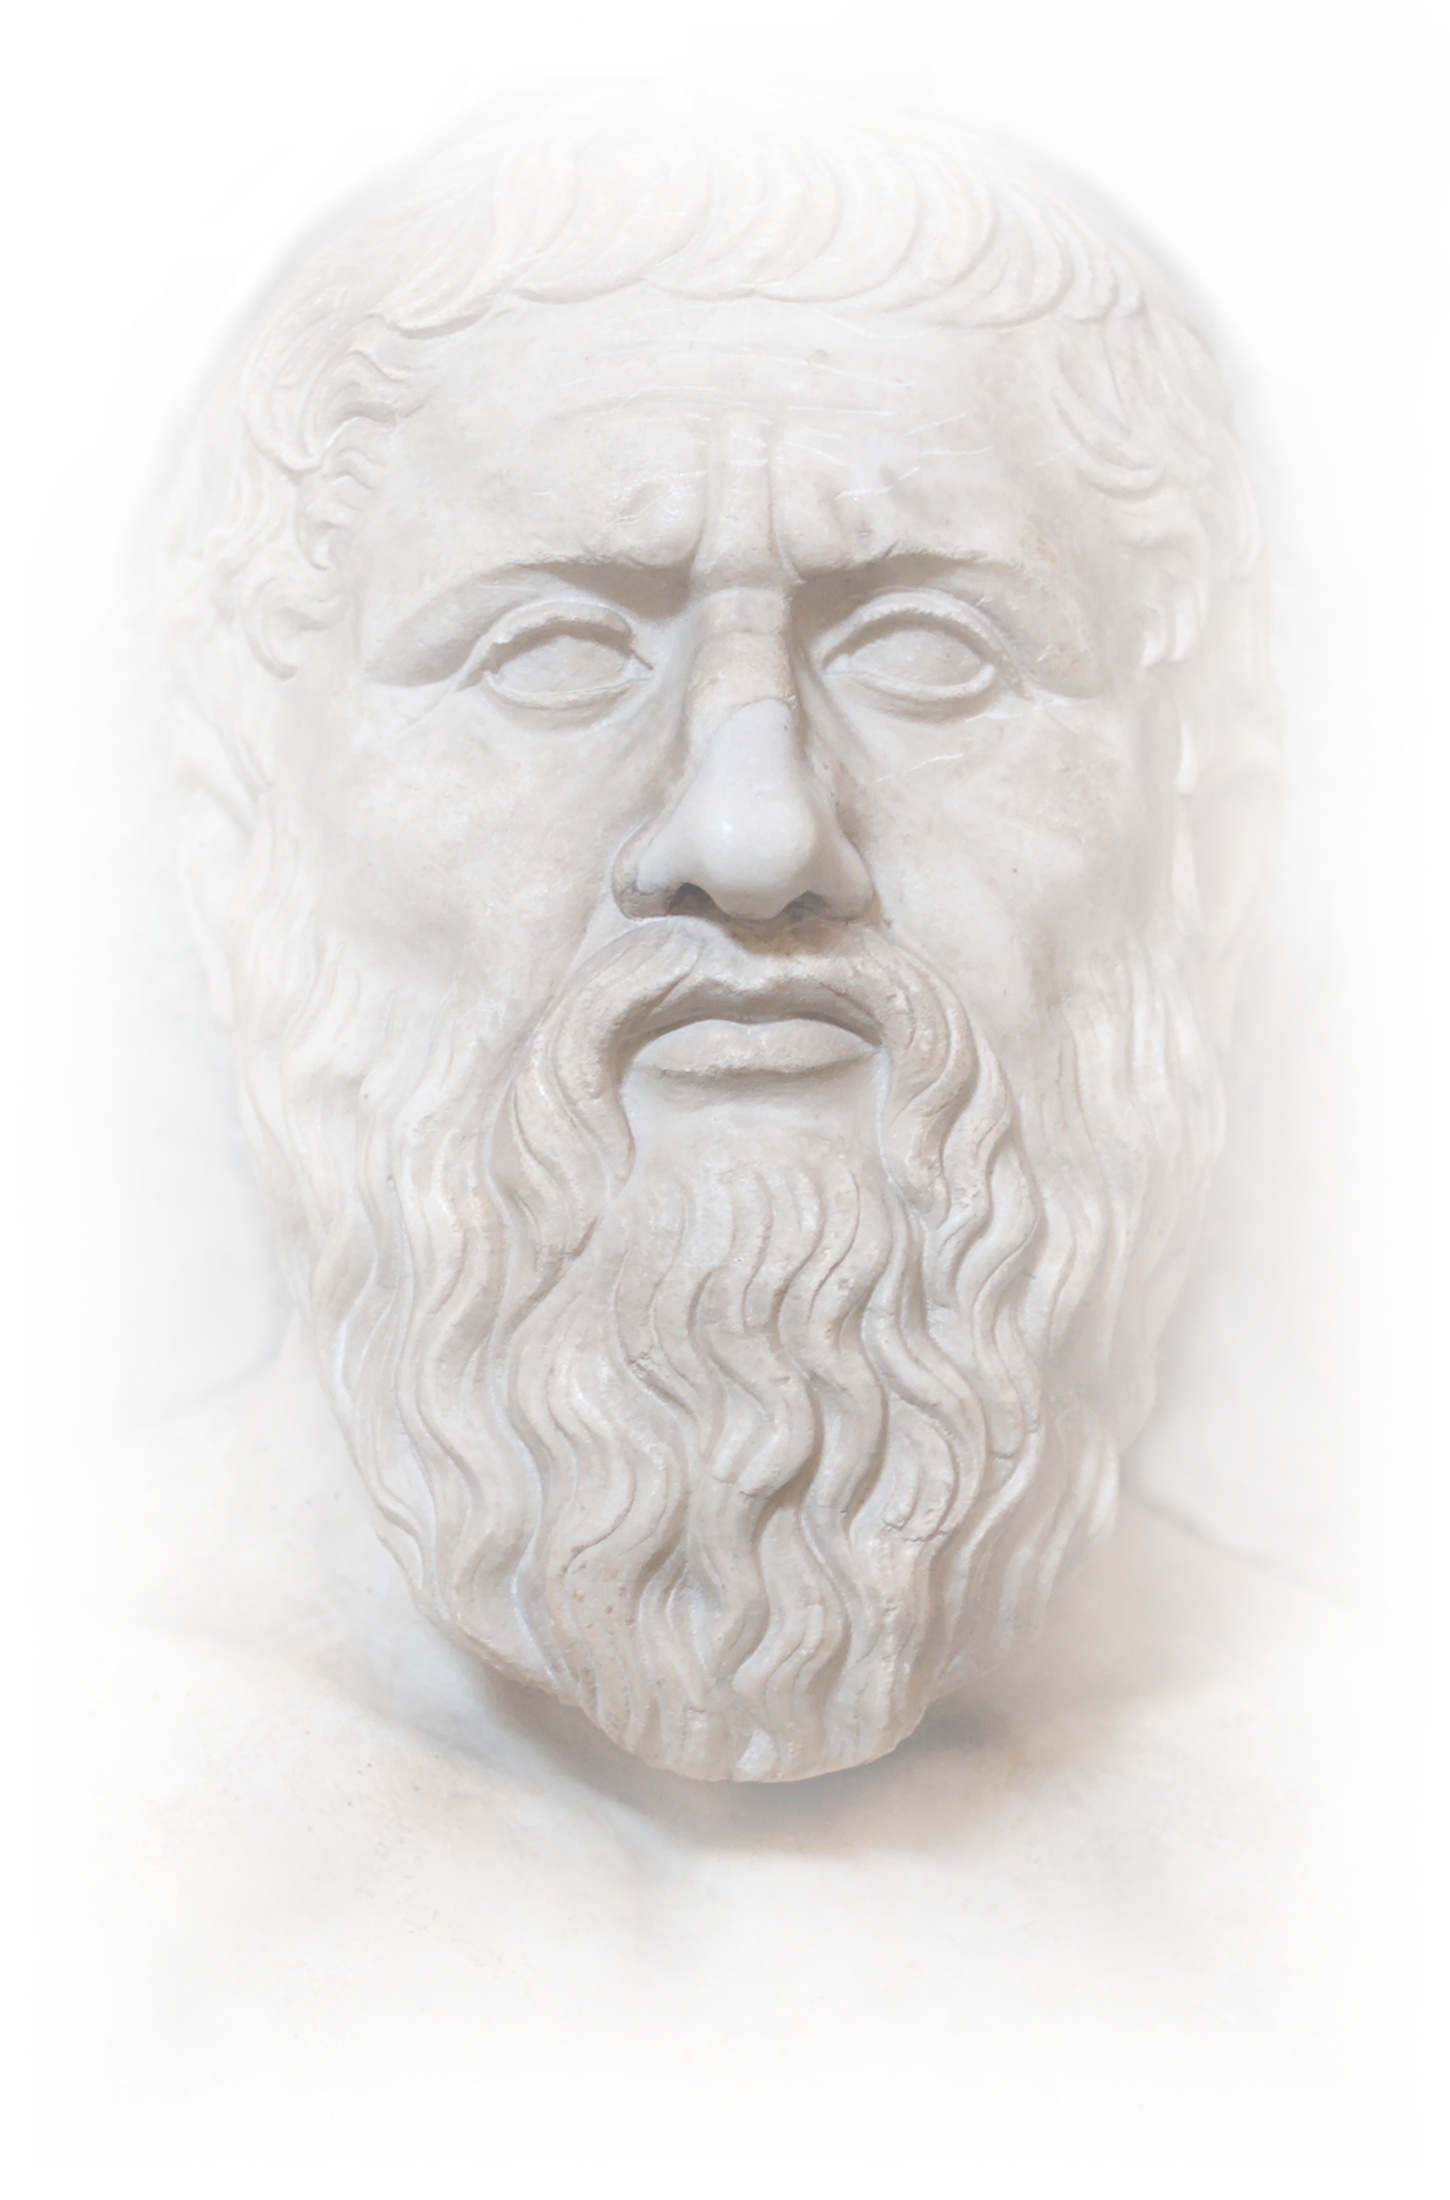
\includegraphics[width=8.5cm]{../resources/jpg/1.6.introduction.to.proofs/plato.jpg}
    \caption*{\emph{Plato.}}
\end{figure}
\pagebreak


% ============================== 1.15 Theorem 1617 ================================
\section{Odd integers of the form $\bm{\zeta ^3 \textbf{ + } 5}$.}
\documentclass[preview]{standalone}
\usepackage{amssymb, amsmath, amsthm}
\usepackage{mathtools}
\usepackage{bm}


\newtheorem{theorem}{Theorem}
\renewcommand\qedsymbol{$\blacksquare$}


\begin{document}


\begin{theorem} %[\textbf{1617}]
    Let \bm{$\zeta$} be an integer. 
    If \bm{$\zeta^3 \textbf{ + } 5$} is odd, 
    then \bm{$\zeta$} is even.
\end{theorem}

\begin{proof}
    By the contrapositive. 
    Suppose that \bm{$\zeta$} were odd. 
    By the definition for odd numbers, 
    there exists an integer \bm{$\gamma$} such that 
    \bm{$\zeta \textbf{ = } 2\gamma \textbf{ + } 1$}. 
    By the Binomial Theorem,
    \begin{equation*}
        \Bigg \{
            \big \langle 2 \gamma + 1 \big \rangle ^3 + 5
        \Bigg \}
            = 
        \Bigg \{
            5 
                + 
            \sum\limits_{\iota=0} ^3 {3 \choose \iota} 
                2 \gamma ^{\langle 3 - \iota \rangle}
        \Bigg \}
            = 
        \Bigg \{
            2 
            \big \langle 4 \gamma ^3 - 6 \gamma ^2 + 3 \gamma + 3 \big \rangle
        \Bigg \}
    \end{equation*}
    The factor 
    \bm{$\big \langle 4 \gamma ^3 \textbf{ - } 6 \gamma ^2 \textbf{ + } 3 \gamma \textbf{ + } 3 \big \rangle$} 
    is an integer because integers are closed on addition and multiplication. 
    Thus, \bm{$\zeta^3 \textbf{ + } 5$} is even, by definition.
\end{proof}


\end{document}
\begin{figure}[h!]
    \centering
    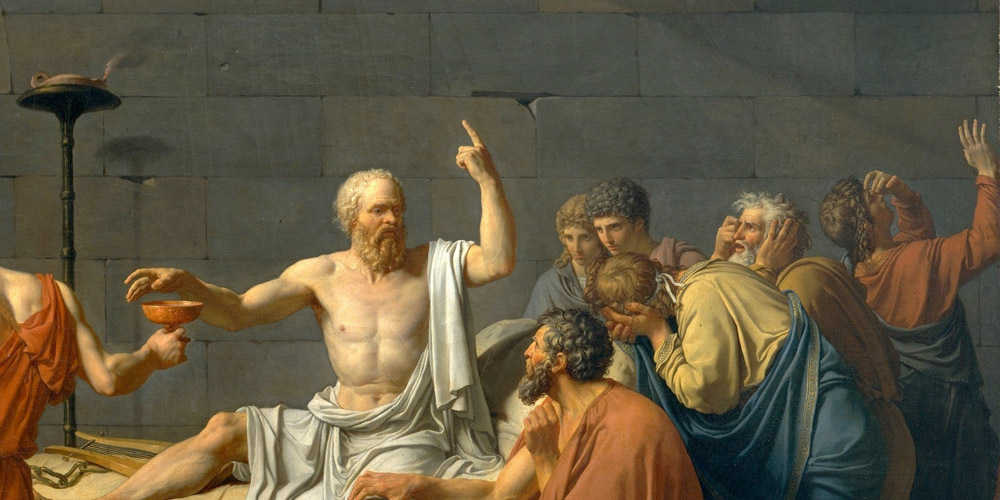
\includegraphics[width=13.25cm]{../resources/jpg/1.6.introduction.to.proofs/socrates.jpg}
    \caption*{\emph{Socrates with hemlock.}}
\end{figure}


% ============================== 1.16 Theorem 1618 ================================
\section{Even numbers of the form $\bm{3 \gamma \textbf{ + } 2}$.}
\documentclass[preview]{standalone}
\usepackage{amssymb, amsthm}
\usepackage{mathtools}
\usepackage{bm}


\newtheorem{theorem}{Theorem}
\renewcommand\qedsymbol{$\blacksquare$}


\begin{document}


\begin{theorem} %[\textbf{1618}]
    Let \bm{$\gamma$} be an integer. 
    If \bm{$3 \gamma \textbf{ + } 2$} is even, 
    then \bm{$\gamma$} is even.
\end{theorem}

\begin{proof}
    By the contrapositive. 
    Suppose \bm{$\gamma$} were odd. 
    By the definition of odd numbers,
    there exist an integer \bm{$\mu$} such that 
    \bm{$\gamma \textbf{ = } 2 \mu \textbf{ + } 1$}. 
    Thus,
    \begin{equation*}
        \Big \langle
            3 \big[ 2 \mu + 1 \big] + 2 
        \Big \rangle
            = 
        \Big \langle
            6 \mu + 5
        \Big \rangle
            =
        \Big \langle
            6 \mu + 4 + 1 
        \Big \rangle
            =
        \Big \langle
            2 \big[ 3 \mu + 2 \big] + 1
        \Big \rangle
    \end{equation*} 
    The factor \bm{$\big[ 3 \mu \textbf{ + } 2 \big]$} is an integer, 
    since integers are closed on addition and multiplcation. 
    Thus, \bm{$3\gamma \textbf{ + } 2$} is odd, by definition.
\end{proof}


\end{document}
\pagebreak


% ============================== 1.17 Theorem 1625 ================================
\section{$\bm{\rho}$ does not exist.}
\documentclass[preview]{standalone}
\usepackage{amssymb, amsthm}
\usepackage{mathtools}
\usepackage{bm}
\usepackage{xcolor}


\newtheorem{theorem}{Theorem}
\renewcommand\qedsymbol{$\blacksquare$}


\begin{document}


\begin{theorem} %[\textbf{1625}]
    There does not exist a rational number \bm{$\rho$} such that 
    \bm{$\rho^3 + \rho + 1 = 0$}.
\end{theorem}

\begin{proof}
    For the purpose of contradiction, 
    assume that there exists a rational number \bm{$\rho$} satisfying the equation \bm{$\rho^3 + \rho + 1 = 0$}. 
    By the definition for rational numbers, 
    there exist integers \bm{$\alpha$} and \bm{$\beta$} (\bm{$\beta$} is nonzero,) such that 
    \begin{equation*}
        \left( 
            \rho ^3 + \rho + 1 
        \right) 
            = 
        \left( 
            \frac{\alpha^3}{\beta^3} + \frac{\alpha}{\beta} + 1 
        \right) 
            = 
        0
    \end{equation*}
    By the additive equality property for equations, that is
    \begin{equation*}
        \frac{\alpha^3}{\beta^3} 
            = 
        \left(
            -1 - \frac{\alpha}{\beta}
        \right)
    \end{equation*}
    It is possible to derive \bm{$\rho^2$} from \bm{$\rho^3$} 
    by multiplying \bm{$\rho^3$} by the multiplicative inverse for \bm{$\rho$}. 
    By the multiplicative equality property for equations,
    \begin{equation*}
        \frac{\alpha^3}{\beta^3} \cdot \frac{\beta}{\alpha}
            =
        \left(
            -1 - \frac{\alpha}{\beta}
        \right) 
            \cdot 
        \frac{\beta}{\alpha} 
            =
        \left\{
            \frac{-\beta}{\alpha} 
                - 
            \frac{\alpha \beta}{\beta \alpha}
        \right\}
    \end{equation*}
    Thus, by the field axioms, \bm{$\rho^2$} is
    \begin{equation*}
        \left\{
            \frac{-\beta}{\alpha} 
                - 
            \frac{\alpha \beta}{\beta \alpha}
        \right\}
            = 
        \left(
            \frac{-\beta - \alpha}{\alpha}
        \right)
            = 
        -1 
            \cdot 
        \left( 
            \frac{\beta + \alpha}{\alpha}
        \right)
    \end{equation*}
    Applying the square root to \bm{$\rho^2$} gives the identity for \bm{$\rho$}
    \begin{equation*}
        \sqrt{ \frac{\alpha^2}{\beta^2} } 
            =
        \sqrt{ -1 \cdot \left( \frac{\beta + \alpha}{\alpha} \right) } 
            =
        i \cdot \sqrt{ \left( \frac{\beta + \alpha}{\alpha} \right) }
    \end{equation*}
    \bm{$\rho$} is imaginary and rational. 
    Thus, the negation of the hypothesis implies a contradiction. 
    In other words, \bm{$\rho$} does not exist.
\color{lightgray} \end{proof}



\end{document}
\sep
\begin{figure}[h!]
    \centering
    
\includegraphics[width=10cm]{../resources/jpg/1.6.introduction.to.proofs/know_thyself.jpg}
    \caption*{\emph{Know thyself.}}
\end{figure} 
\pagebreak
\thispagestyle{empty}


\end{document}